\documentclass[../main.tex]{subfiles}

\begin{document}
  \noindent{Archons are celestials from a lawful good-aligned plane.}\\
  \noindent{Archons speak Celestial, Infernal, and Draconic, but can speak with almost any creature because of their tongues ability.}

  \dndsection{COMBAT}
  \noindent{Archons generally prefer to meet a foe head-on if it is prudent to do so, but if outmatched, they do what they can to even the odds (usually by employing hit-and run tactics or standing off and engaging a foe with magic before moving into melee).}\\
  \indent{\textbf{Archon Traits:} An archon possesses the following traits (unless otherwise noted in a creature’s entry).}\\
  \indent{--Darkvision out to 60 feet and low-light vision.}\\
  \indent{--\textit{Aura of Menace (Su):} A righteous aura surrounds archons that fight or get angry. Any hostile creature within a 20-foot radius of an archon must succeed on a Will save to resist its effects. The save DC varies with the type of archon, is Charisma-based, and includes a +2 racial bonus. Those who fail take a –2 penalty on attacks, AC, and saves for 24 hours or until they successfully hit the archon that generated the aura. A creature that has resisted or broken the effect cannot be affected again by the same archon’s aura for 24 hours.}\\
  \indent{--Immunity to electricity and petrification.}\\
  \indent{-- +4 racial bonus on saves against poison.}\\
  \indent{--\textit{Magic Circle against Evil (Su):} A magic circle against evil effect always surrounds an archon (caster level equals the archon’s Hit Dice). (The defensive benefits from the circle are not included in an archon’s statistics block.)}\\
  \indent{--\textit{Teleport (Su):} Archons can use greater teleport at will, as the spell (caster level 14th), except that the creature can transport only itself and up to 50 pounds of objects.}\\
  \indent{--\textit{Tongues (Su):} All archons can speak with any creature that has a language, as though using a tongues spell (caster level 14th). This ability is always active.}
  \vspace{6cm}\vfill
  \dndsection{LANTERN ARCHON}
  \begin{table}[H]
    \centering
    \begin{tabular}{lp{12em}}
       & \textbf{Small Outsider (Arcon, Extraplanar, Good, Lawful)} \\
       \textbf{Hit Dice:} & 1d8 (4hp) \\
       \textbf{Initiative:} & +4 \\
       \textbf{Speed:} & Fly 60 ft. (perfect)(12 squares) \\
       \textbf{Armor Class:} & 15 (+1 size, +4 natural), touch 11, flat-footed 15 \\
       \textbf{Base Attack/Grapple:} & +1/-8 \\
       \textbf{Attack:} & Light ray +2 ranged touch (1d6) \\
       \textbf{Full Attack:} & 2 light rays +2 ranged touch (1d6) \\
       \textbf{Space/Reach:} & 5 ft./5 ft. \\
       \textbf{Special Attacks:} & Spell-like abilities \\
       \textbf{Special Qualities:} & Aura of menace, damage reduction 10/evil and magic, darkvision 60 ft., immunity to electricity and petrification, magic circle against evil, teleport, tongues \\
       \textbf{Saves:} & Fort +2 (+6 against poison), Ref +2, Will +2 \\
       \textbf{Abilities:} & Str 1, Dex 11, Con 10, Int 6, Wis 11, Cha 10 \\
       \textbf{Skills:} & Concentration +4, Diplomacy +4, Knowledge (the planes) +2, Listen +4, Sense Motive +4, Spot +4 \\
       \textbf{Feats:} & Improved initiative \\
       \textbf{Environment:} & Seven Mounting Heavens of Celestia \\
       \textbf{Organization:} & Solitary, pair, or squad (3-5) \\
       \textbf{Challenge Rating:} & 2 \\
       \textbf{Treasure:} & None \\
       \textbf{Alignment:} & Always lawful good \\
       \textbf{Advancement:} & 2-4 HD (Small) \\
       \textbf{Level Adjustment:} & -- \\
    \end{tabular}
  \end{table}

  \noindent{\textit{A ball of glowing light floats toward you.}}

  \noindent{Lantern archons appear as floating balls of light that glow about as brightly as a torch. Only their destruction can extinguish the glow, though they can try to hide it.}\\
  \indent{Lantern archons are very friendly and usually eager to give what assistance they can. However, their bodies are just gaseous globes, and they are much too weak to render any material aid. Lantern archons speak in soft, musical voices.}\\
  \dndsubsection{Combat}
  \noindent{A lantern archon has little reason to get within melee range. It usually hovers just close enough to bring the enemy within its aura of menace, then blasts away with its light rays. Lantern archons prefer to concentrate on a single opponent, seeking to reduce enemy numbers quickly.}\\
  \indent{\textbf{Aura of Menace (Su):} Will DC 12 negates.}\\
  \indent{\textbf{Light Ray (Ex):} A lantern archon’s light rays have a range of 30 feet. This attack overcomes damage reduction of any type.}\\
  \indent{\textbf{Spell-Like Abilities:} At will--\textit{aid}, \textit{detect evil}, \textit{continual flame}. Caster level 3rd.}

  \dndsection{HOUND ARCHON}
  \noindent{\textit{A powerfully build humanoid with the head of a dog appears both serene and ready for action, with a greatsword strapped to its broad back and an expression that indicates intelligence and protectiveness.}} \\

  \noindent{Hound archons look like well-muscled humans with canine heads. They seek to defend the innocent and help the helpless against evil.}\\
  \indent{Their broad shoulders and meaty fists mark hound archons as able combatants. Likewise, their legs indicate that fleeing enemies won't get very far.}

  \begin{table*}[H]
    \centering
    \begin{tabular}{p{9em}p{12em}p{16em}}
       & \textbf{Hound Archon} & \textbf{Hound Archon Hero, 11th-Level Paladin} \\
       & \textbf{Medium Outsider (Archon, Extraplanar, Good, Lawful)} & \textbf{Medium Outsider (Archon, Extraplanar, Good, Lawful)} \\
      \rowcolor[HTML]{FFCE93}
      \textbf{Hit Dice:} & 6d8+6 (33 hp) & 6d8+18 plus 11d10+33 (143 hp) \\
      \textbf{Initiative:} & +4 & +4 \\
      \rowcolor[HTML]{FFCE93}
      \textbf{Speed:} & 40 ft. (8 squares) & 30 ft. in full plate armor (6 squares); base speed 40 ft. \\
      \textbf{Armor Class:} & 19 (+9 natural), touch 10, flat-footed 19 & 30 (+9 natural, +11 +3 full plate armor), touch 10, flat-footed 30 \\
      \rowcolor[HTML]{FFCE93}
      \textbf{Base Attack/Grapple:} & +6/+8 & +17/+22 \\
      \textbf{Attack:} & Bite +8 melee (1d8+2) or greatsword +8 melee (2d6+3/19–20) & +2 cold iron greatsword +25 melee (2d6+9/19–20) or bite +22 melee (1d8+5) \\
      \rowcolor[HTML]{FFCE93}
      \textbf{Full Attack:} & Bite +8 melee (1d8+2) and slam +3 melee (1d4+1); or greatsword +8/+3 melee (2d6+3/19–20) and bite +3 melee (1d8+1) & +2 cold iron greatsword +25/+20/+15/+10 melee (2d6+9/19–20) and bite +17 melee (1d8+2); or bite +22 melee (1d8+5) and slam +17 melee (1d4+2) \\
      \textbf{Space/Reach:} & 5 ft./5 ft. & 5 ft./5 ft. \\
      \rowcolor[HTML]{FFCE93}
      \textbf{Special Attacks:} & Spell-like abilities & Smite evil, spells, spell-like abilities, turn undead 6/day \\
      \textbf{Special Qualities:} & Aura of menace, change shape, damage reduction 10/evil, darkvision 60 ft., immunity to electricity and petrification, magic circle against evil, scent, spell resistance 16, teleport, tongues & Aura of menace, change shape, damage reduction 10/evil, darkvision 60 ft., immunity to electricity and petrification, magic circle against evil, paladin abilities, scent, spell resistance 27, teleport, tongues \\
      \rowcolor[HTML]{FFCE93}
      \textbf{Saves:} & Fort +6 (+10 against poison), Ref +5, Will +6 & Fort +18 (+22 against poison), Ref +11, Will +13 \\
      \textbf{Abilities:} & Str 15, Dex 10, Con 13, Int 10, Wis 13, Cha 12 & Str 21, Dex 10, Con 16, Int 8, Wis 14, Cha 16 \\
      \rowcolor[HTML]{FFCE93}
      \textbf{Skills:} & Concentration +10, Diplomacy +3, Hide +9*, Jump +15, Listen +10, Move Silently +9, Sense Motive +10, Spot +10, Survival +10* (+12 following tracks) & Concentration +20, Diplomacy +19, Hide +2*, Jump +0, Listen +10, Ride +14, Sense Motive +19, Spot +10, Survival +2* \\
      \textbf{Feats:} & Improved Initiative, Power Attack, Track & Improved Initiative, Leadership, Mounted Combat, Ride-By Attack, Track, Weapon Focus (greatsword)  \\
      \rowcolor[HTML]{FFCE93}
      \textbf{Environment:} & A lawful good-aligned plane & A lawful good-aligned plane \\
      \textbf{Organization:} & Solitary, pair, or squad (3–5) & Solitary or with juvenile bronze dragon \\
      \rowcolor[HTML]{FFCE93}
      \textbf{Challenge Rating:} & 4 & 16 \\
      \textbf{Treasure:} & No coins; double goods; standard items & Standard \\
      \rowcolor[HTML]{FFCE93}
      \textbf{Alignment:} & Always lawful good & Always lawful good \\
      \textbf{Advancement:} & 7–9 HD (Medium); 10–18 HD (Large) & By character class \\
      \rowcolor[HTML]{FFCE93}
      \textbf{Level Adjustment:} & +5 & +5 \\
    \end{tabular}
  \end{table*}

  \dndsubsection{Combat}
  \noindent{Hound archons prefer to attack with their natural weapons but occasionally use greatswords.}\\
  \indent{A hound archon’s natural weapons, as well as any weapons it wields, are treated as good-aligned and lawful-aligned for the purpose of overcoming damage reduction.}\\
  \indent{\textbf{Spell-Like Abilities:} At will—aid, continual flame, detect evil, message. Caster level 6th.}\\
  \indent{\textbf{Aura of Menace (Su):} Will DC 16 negates.}\\
  \indent{\textbf{Change Shape (Su):} A hound archon can assume any canine form of Small to Large size. While in canine form, the hound archon loses its bite, slam, and greatsword attacks, but gains the bite attack of the form it chooses. For the purposes of this ability, canines include any doglike or wolflike animal of the animal type.}\\
  \indent{\textbf{Skills:} *While in canine form, a hound archon gains a +4 circumstance bonus on Hide and Survival checks.}

  \dndsubsection{Hound Archon Hero}
  \noindent{The hound archon hero is a mighty champion of justice, devoted to the pursuit and destruction of evil in all its forms.}
  \dndsubsection{COMBAT}
  \noindent{Hound archon heroes have over time developed a love for their weapons. They prefer to use their holy greatswords over their bite and slam attacks.}\\
  \indent{\textbf{Spell-Like Abilities:} At will—aid, continual flame, detect evil, message. Caster level 6th.}\\
  \indent{\textbf{Aura of Menace (Su):} The save DC for the hound archon hero’s aura of menace (DC 18) is adjusted for its higher Charisma score.}\\
  \indent{\textbf{Smite Evil (Su):} Three times per day a hound archon hero can make a normal melee attack with a +3 bonus that deals an extra 11 points of damage against an evil foe.}\\
  \indent{\textbf{Change Shape (Su):} A hound archon hero can assume any canine form of Small to Large size. While in canine form, the hound archon loses its bite, slam, and greatsword attacks, but gains the bite attack of the form it chooses. For the purposes of this ability, canines include any doglike or wolflike animal of the animal type.}\\
  \indent{\textbf{Skills:} *While in canine form, a hound archon hero gains a +4 circumstance bonus on Hide and Survival checks.}\\
  \indent{\textbf{Paladin Abilities:} Aura of courage, aura of good, detect evil, divine grace, divine health, lay on hands (33 points/day), remove disease 2/week, special mount (juvenile bronze dragon).}\\
  \indent{\textit{Typical Paladin Spells Prepared} (2/2; save DC 12 + spell level): 1st--\textit{divine favor}, \textit{protection from evil}; 2nd--\textit{bull’s strength}, \textit{eagle’s splendor}.}\\
  \indent{\textit{Possessions: +3 full plate armor, +2 cold iron greatsword.}}

  \dndsubsection{HOUND ARCHON HERO MOUNTS}
  \noindent{In the course of their adventures, many hound archon heroes befriend bronze dragons, which may come to serve as their mounts. The relationship between these mounts and their celestial riders goes beyond even the special bond between paladin and mount. The dragon and the archon are naturally allies and friends, as can be expected of two powerful servants of cosmic justice. The juvenile bronze dragon mount gains 2 additional HD, 4 points of Strength, an additional 4 points of natural armor, improved evasion, and +10 feet to speed in all its movement forms. The dragon cannot, however, command other creatures of its type as other kinds of paladin mounts can.} \\

  \dndsubsection{HOUND ARCHONS AS CHARACTERS}
  \noindent{Hound archon characters possess the following racial traits.} \\
  \indent{-- +4 Strength, +2 Constitution, +2 Wisdom, +2 Charisma.} \\
  \indent{--Medium size.} \\
  \indent{--A hound archon’s base land speed is 40 feet.} \\
  \indent{--Racial Hit Dice: A hound archon begins with six levels of outsider, which provide 6d8 Hit Dice, a base attack bonus of +6, and base saving throw bonuses of Fort +5, Ref +5, and Will +5.} \\
  \indent{--Racial Skills: A hound archon’s outsider levels give it skill points equal to 9 × (8 + Int modifier). Its class skills are Concentration, Hide, Jump, Listen, Move Silently, Sense Motive, Spot, and Survival.} \\
  \indent{--Racial Feats: A hound archon’s outsider levels give it three feats.} \\
  \indent{-- +9 natural armor bonus.} \\
  \indent{--Natural Weapons: Bite (1d8) and slam (1d4).} \\
  \indent{--Archon Traits (see page 16): Darkvision 60 ft., low-light vision, aura of menace (Will DC 15 + character’s Cha modifier), immunity to electricity and petrification, +4 racial bonus on saves against poison, magic circle against evil, teleport, tongues.} \\
  \indent{--Special Attacks: Spell-like abilities.} \\
  \indent{--Special Qualities: Change shape, damage reduction 10/evil, scent, spell resistance equal to 16 + class levels.} \\
  \indent{--Automatic Languages: Celestial. Bonus Languages: Common, Draconic, Infernal.} \\
  \indent{--Favored class: Ranger.} \\
  \indent{--Level adjustment +5.} \\

  \dndsection{TRUMPET ARCHON}
  \begin{table}[H]
    \centering
    \begin{tabular}{p{9em}p{12em}}
       & \textbf{Medium Outsider (Archon, Extraplanar, Good, Lawful)} \\
      \textbf{Hit Dice:} & 12d8+72 (126 hp) \\
      \textbf{Initiative:} & +7 \\
      \textbf{Speed:} & 40 ft. (8 squares), fly 90 ft. (good) \\
      \textbf{Armor Class:} & 27 (+3 Dex, +14 natural), touch 13, flat-footed 24 \\
      \textbf{Base Attack/Grapple:} & +12/+17 \\
      \textbf{Attack:} & +4 greatsword +21 melee (2d6+11/19–20) \\
      \textbf{Full Attack:} & +4 greatsword +21/+16/+11 melee (2d6+11/19–20) \\
      \textbf{Space/Reach:} & 5 ft./5 ft. \\
      \textbf{Special Attacks:} & Spell-like abilities, spells, trumpet \\
      \textbf{Special Qualities:} & Aura of menace, damage reduction 10/evil, darkvision 60 ft., immunity to electricity and petrification, magic circle against evil, spell resistance 29, teleport, tongues \\
      \textbf{Saves:} & Fort +14 (+18 against poison), Ref +11, Will +11 \\
      \textbf{Abilities:} & Str 20, Dex 17, Con 23, Int 16, Wis 16, Cha 16 \\
      \textbf{Skills:} & Concentration +21, Diplomacy +20, Escape Artist +18, Handle Animal +18, Knowledge (any one) +18, Listen +18, Move Silently +18, Perform (wind instruments) +18, Ride +20, Sense Motive +18, Spot +18, Use Rope +3 (+5 with bindings) \\
      \textbf{Feats:} & Blind-Fight, Cleave, Combat Reflexes, Improved Initiative, Power Attack \\
      \textbf{Environment:} & A lawful good-aligned plane \\
      \textbf{Organization:} & Solitary, pair, or squad (3–5) \\
      \textbf{Challenge Rating:} & 14 \\
      \textbf{Treasure:} & No coins; double goods; standard items \\
      \textbf{Alignment:} & Always lawful good \\
      \textbf{Advancement:} & 13–18 HD (Medium); 19–36 HD (Large) \\
      \textbf{Level Adjustment:} & +8 \\
    \end{tabular}
  \end{table}

  \noindent{\textit{Appearing as a green winged elf of supernatural goodness and beuaty, the creature raises a massive silver trumpet and sounds a blast of piercing soul-wrenching music.}\\

  \noindent{Trumpet archons serve as celestial messengers and heralds, though their martial skills are considerable. Each carries a gleaming silver trumpet about 6 feet long.}

  \dndsubsection{Combat}
  \noindent{A trumpet archon usually disdains physical combat, preferring to obliterate foes with spells quickly and return to its duties. If forced into an extended battle, it sounds its trumpet and attacks with a vengeance.} \\
  \indent{A trumpet archon’s natural weapons, as well as any weapons it wields, are treated as good-aligned and lawful-aligned for the purpose of overcoming damage reduction.} \\
  \indent{\textbf{Spell-Like Abilities:} At will—detect evil, continual flame, message. Caster level 12th.} \\
  \indent{\textbf{Aura of Menace (Su):} Will DC 21 negates.} \\
  \indent{\textbf{Spells:} Trumpet archons can cast divine spells as 14th-level clerics. A trumpet archon has access to two of the following domains: Air, Destruction, Good, Law, or War (plus any others from its deity). The save DCs are Wisdom-based.} \\
  \indent{\textit{Typical Cleric Spells Prepared} (6/7/7/6/5/4/4/3; DC 13 + spell level): 0--\textit{detect magic}, \textit{light}, \textit{purify food and drink}, \textit{read magic}, \textit{resistance} (2); 1st--\textit{bless} (2), \textit{divine favor} (2), \textit{protection from chaos*}, \textit{sanctuary}, \textit{shield of faith}; 2nd--\textit{aid*}, \textit{bull’s strength} (2), \textit{consecrate}, \textit{lesser restoration}, \textit{owl’s wisdom} (2); 3rd--\textit{daylight}, \textit{invisibility purge}, \textit{magic circle against chaos*}, \textit{magic vestment}, \textit{protection from energy} (2); 4th--\textit{dismissal}, \textit{divine power}, \textit{holy smite*}, \textit{neutralize poison}, \textit{spell immunity}; 5th--\textit{dispel evil*}, \textit{mass cure light wounds}, \textit{plane shift}, \textit{raise dead}; 6th--\textit{blade barrier*}, \textit{banishment}, \textit{heal}, \textit{undeath to death}; 7th--\textit{dictum*}, \textit{holy word}, \textit{mass cure serious wounds}.} \\
  \indent{*Domain spell. Domains: Good and Law.} \\
  \indent{\textbf{Trumpet (Su):} An archon’s trumpet produces music of utter clarity, piercing beauty, and, if the trumpet archon wills it, paralyzing awe. All creatures except archons within 100 feet of the blast must succeed on a DC 19 Fortitude save or be paralyzed for 1d4 rounds. The save DC is Charisma-based. The archon can also command its trumpet to become a \textit{+4 greatsword} as a free action.} \\
  \indent{If a trumpet is ever stolen, it becomes a chunk of useless metal until the owner can recover it. Woe betide any thief caught with one.} \\

  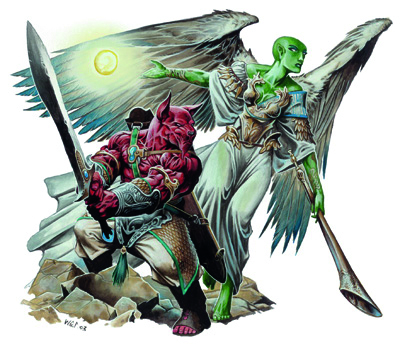
\includegraphics[width=\columnwidth]{Archon}
}
\end{document}
